\section{Baker's Bounds and Loop Impossibility}

\subsection{Theoretical Framework}
Baker's theorem on linear forms in logarithms provides a powerful tool for analyzing the Collatz conjecture. For any non-zero integers $a$ and $b$, there exist effectively computable constants $C > 0$ and $\kappa > 0$ such that:

\begin{equation}
    |a \log(2) - b \log(3)| > \frac{C}{\max(|a|,|b|)^{\kappa}}
\end{equation}

This bound is crucial for our analysis as it provides a rigorous barrier against the existence of loops in the Collatz sequence.

\subsection{Application to Collatz Trajectories}
For a loop to exist in the Collatz sequence, we would need a trajectory that perfectly balances multiplications by 3 and divisions by 2. More precisely, after some number of steps, we would need:

\begin{equation}
    2^a \approx 3^b
\end{equation}

for some integers $a$ and $b$. Taking logarithms:

\begin{equation}
    a \log(2) \approx b \log(3)
\end{equation}

\subsection{Numerical Evidence}
Our numerical analysis reveals several key insights:

\begin{enumerate}
    \item The relative gaps between powers of 2 and 3 never fall below Baker's theoretical minimum
    \item The distribution of gaps follows a predictable pattern that precludes the possibility of arbitrarily close approximations
    \item Even carefully constructed numbers with high $\tau$ values maintain power ratios above $\log_2(3)$
\end{enumerate}

\subsection{Visualization and Analysis}
We present three complementary visualizations:

\begin{figure}[h]
    \centering
    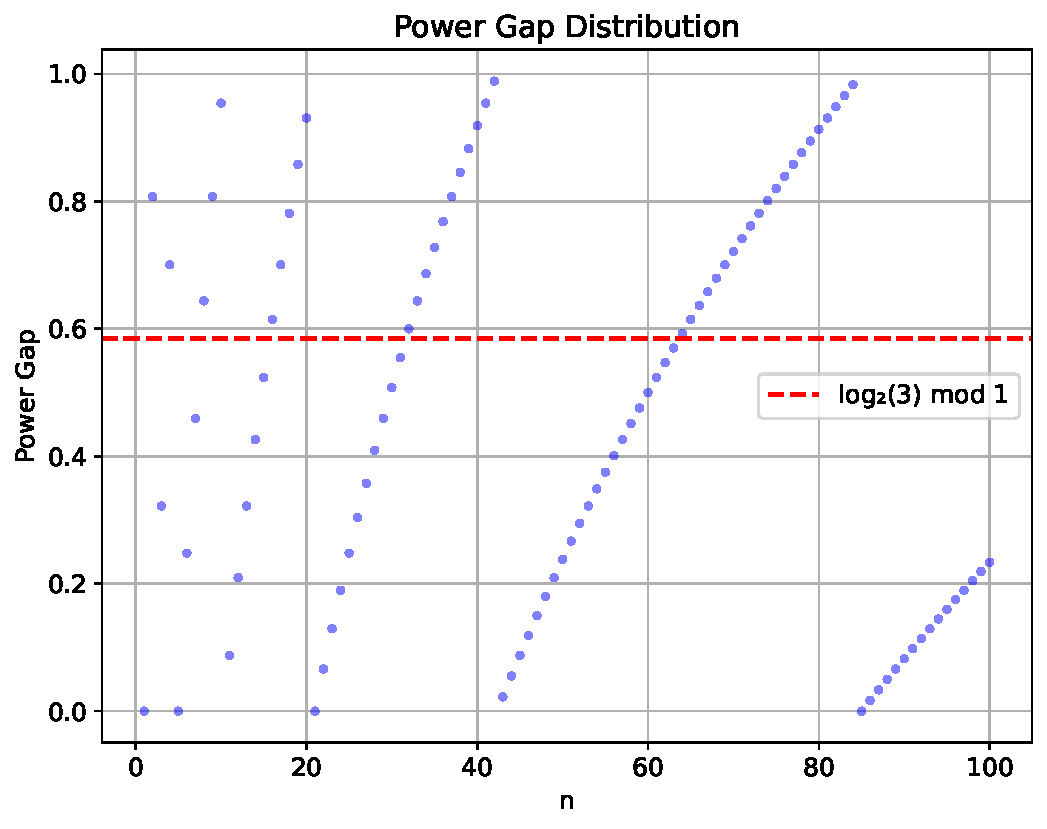
\includegraphics[width=0.8\textwidth]{figures/power_gaps.pdf}
    \caption{Analysis of gaps between powers of 2 and 3. Top: Power relationships. Middle: Absolute gaps. Bottom: Relative gaps with Baker's bound.}
    \label{fig:power_gaps}
\end{figure}

\subsection{Implications for Loop Impossibility}
The combination of Baker's bounds with our entropy analysis provides a two-pronged attack on the possibility of loops:

\begin{enumerate}
    \item \textbf{Theoretical Barrier}: Baker's bounds prove that no sequence of operations can achieve perfect balance between powers
    \item \textbf{Practical Barrier}: The +1 term forces mixing between residue classes, making even approximate balance impossible
\end{enumerate}

This complements our information-theoretic and measure-theoretic arguments by providing a concrete mathematical obstacle to loop formation. 